\documentclass{article}

% if you need to pass options to natbib, use, e.g.:
%     \PassOptionsToPackage{numbers, compress}{natbib}
% before loading neurips_2019

% ready for submission
% \usepackage{neurips_2019}

% to compile a preprint version, e.g., for submission to arXiv, add add the
% [preprint] option:
%     \usepackage[preprint]{neurips_2019}

% to compile a camera-ready version, add the [final] option, e.g.:
\usepackage[final]{neurips_2019}

% to avoid loading the natbib package, add option nonatbib:
%     \usepackage[nonatbib]{neurips_2019}

\usepackage[utf8]{inputenc} % allow utf-8 input
\usepackage[T1]{fontenc}    % use 8-bit T1 fonts
\usepackage{hyperref}       % hyperlinks
\usepackage{url}            % simple URL typesetting
\usepackage{booktabs}       % professional-quality tables
\usepackage{amsfonts}       % blackboard math symbols
\usepackage{nicefrac}       % compact symbols for 1/2, etc.
\usepackage{microtype}      % microtypography
\usepackage{array}
\newcolumntype{L}{>{\centering\arraybackslash}m{7.5cm}}
% for importing images
\usepackage{graphicx}
\graphicspath{
	{graphics/}
}

\usepackage{pythonhighlight}

\title{Mimic: Character Based Chatbot}

% The \author macro works with any number of authors. There are two commands
% used to separate the names and addresses of multiple authors: \And and \AND.
%
% Using \And between authors leaves it to LaTeX to determine where to break the
% lines. Using \AND forces a line break at that point. So, if LaTeX puts 3 of 4
% authors names on the first line, and the last on the second line, try using
% \AND instead of \And before the third author name.

\author{%
	Nirvan S P Theethira\\
	%  Department of Computer Science\\
	%  University of Colorado Boulder\\
	\texttt{nith5605@colorado.edu} \\
	\And
	Charlie Carlson\\
	%  Department of Computer Science\\
	%  University of Colorado Boulder\\
	\texttt{chca0914@colorado.edu} \\
	\And
	Ketan Ramesh\\
	\texttt{kerk1228@colorado.edu} \\
	\And
	Pramod Venkatesh Kulkarni\\
	%  Department of Computer Science\\
	%  University of Colorado Boulder\\
	\texttt{prku8035@colorado.edu} \\
}

\begin{document}
	
	\maketitle
	
	\begin{abstract}
		In this project we explored the problem of creating a chatbot that could mimic a popular television character's personality, Joey from Friends.
		Our dataset was extracted directly from the Friends scripts from each season. 
		We worked with two different neural network models which we trained on the same dataset: a sequence-to-sequence model and a transformer model. 
		To evaluate our models' performance we considered automatic metrics often used to evaluate translation bots and a human based metric inspired by the Turing test.
		Not surprisingly, neither model performed well with respect to the automatic metrics.
		Moreover, we found that both models failed to consistently convince a human tester that their responses captured the personality of Joey.
		We review a collection of troublesome instances for each model and theorize ways in which each model could be improved.
		We conclude that both models had only minor success but it may be interesting to experiment with slightly more complex models and different datasets. 
	\end{abstract}
	
	\section{Introduction}
		A chatbot is a program that provides conversational output in response to user input.
	They have many applications such as customer support interfaces, general question answering services, translation apps and virtual assistants.
	A common goal for chatbots is to simulate a human like interaction for the user.
	To this end many researches have investigated creating chatbots with "personality" or "identity" \cite{Li2016, LINH2019, QianHZXZ17, ZhouHZZL17,NMC2017, 8614104}.
	Such chatbots could drastically improve improve the user experience of nearly all chatbot applications.
	Consider for example the marketability of a witty virtual assistant or an comforting customer service support chatbot.

	Similar to \cite{NMC2017, Li2016, 8614104}, we investigate the related problem of training a neural network to respond like a popular television character, Joey from Friends.
	While general personality qualities might have more wide spread usefulness in real life applications, the ability to mimic well-known personalities such as Joey would also have commercial applications.
	More importantly, such a task can be seen as an important first step to solving the more general problem of training a machine to behave like a human.
	Motivated by this and previous examples, in this work we investigate training two different neural network models act as chatbots with personality.
	In the following sections we will review the dataset we used, the evaluations we performed, the models we considered and then conclude with our results and final thoughts.
	
%	\texttt{We choose Joey because there are existing results in previous papers to compare to, the Friends scripts are publicly available and because we believed that his strong personality would be an easier for our models to successfully mimic.
%	Joey is often described as naive, good-matured, dimwitted, childish and promiscuous. 
%	In a a later section we will explain what dataset was use and how it was created.
%	
%	In this project we considered two neural network models: a sequence-to-sequence model and a transformer model.
%	We picked these models because of their success as general chatbots and translation bots.
%	Our tasks seems to be heavily linked to both of these.
%	Indeed, one way to attempt our tasks would be to perform a two step process which first generates a generic human like response to a statement and then translates it to sound like the normal dialogue Joey.
%	Moreover, we also picked these models because past works have had some success with directly apply them to the same problem \cite{NMC2017, Li2016, 8614104}.
%	We will discuss both models' details, successes, and weaknesses in later sections.
%	
%	To evaluate the performance of our models we considered two types of metrics: automatic metrics and human metrics.
%	The automatic metrics we considered were those which are usually used to evaluate the performance of translation bots: BLEU, ROUGE, METEOR and WER \cite{Papineni:2002:BMA:1073083.1073135, lin-2004-rouge, denkowski:lavie:meteor-wmt:2014}.
%	While there seems to be a heavy relationship between our task and that of machine translation, these metrics are known to consistently be poor measures of performance for personality chatbots \cite{Radz2017, Xing2018, LiuLSNCP16, SerbanLCP15}.
%	Despite their poor performance, these metrics are still often used as a means to understand some aspects a model's success.
%	However, our primary metric of interest is based on human feedback.
%	For a human based metric we designed a test similar to that of the popular Turing test and asked those familiar with the Joey character to answer a series of questions about responses generated by each of our models.
%	We will discuss both types of metrics in a later section.}

	\section{Dataset and Evaluation}
	In this section we review what datasets we used, how we created them and how we evaluated the performance of our models on them.
	\section{Dataset}
\label{sec:dataset}
\begin{figure}[t]
	\begin{center}
		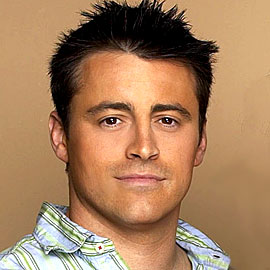
\includegraphics[width=0.4\textwidth]{Matt_LeBlanc_as_Joey_Tribbiani.jpg}
	\end{center}
	\caption{Joey from Friends televisions show. Played by Matt LeBlanc. Image download from Wikipedia and originally from Friends' press release.}
	\label{fig:friends_data_extracted}
\end{figure}
\begin{figure}[t]
	\begin{center}
		\fbox{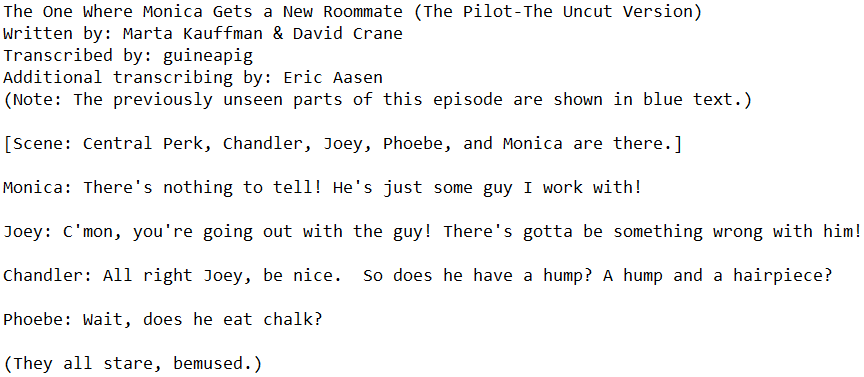
\includegraphics[width=\textwidth]{rawData.PNG}}
	\end{center}
	\caption{Example script content from Friends dataset.}
	\label{fig:friends_data}
\end{figure}

\begin{figure}[h]
	\begin{center}
		\fbox{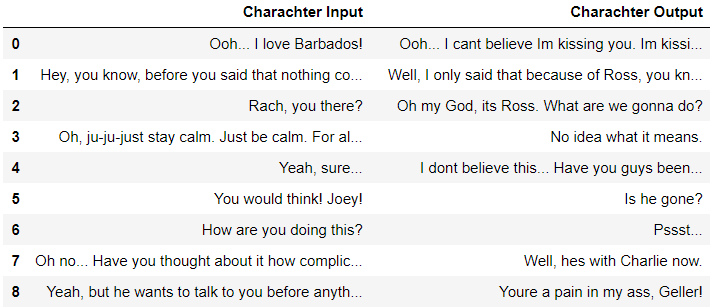
\includegraphics[width=\textwidth]{charachterData.PNG}}
	\end{center}
	\caption{Example of statement response pairs extracted from Friends dataset.}
	\label{fig:friends_data_extracted}
\end{figure}
\begin{figure}[h]
	\begin{center}
		\fbox{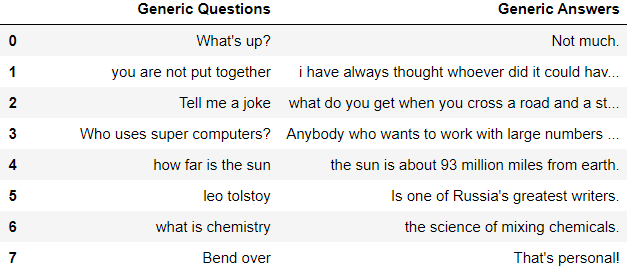
\includegraphics[width=\textwidth]{genericData.PNG}}
	\end{center}
	\caption{Example of statement response pairs extracted from the generic questions and answers dataset.}
	\label{fig:qa_data_extracted}
\end{figure}

To create the personality based chatbot, we first needed a personality to mimic. 
Ideally the personality would be familiar to a large number of people and there would be a large amount of freely available data.
For these reasons we starting looking at characters from popular television shows with multiple seasons.
Moreover, we surmised that the show's writers would have developed a strong and identifiable character personality over the span of several seasons.
We expceted such a personality to be much easier to mimic.
%This gives each character a distinct personality that could be mimicked in a chatbot. 
We also considered movie characters but ultimately, the data available for a movie character was sufficiently smaller than that of a television show character.
%TV show transcripts also offer a larger dataset.

For this project, Friends was chosen as the television show and Joey Tribbiani was chosen as the character. 
We choose Friends because the data was available, the show is popular and it has many seasons.
Joey was chosen to mimic specifically because as has a very distinctive personality in the show. 
For those not familiar the show, Joey can be described as naive, sarcastic, loving, misogynistic, promiscuous and loud.

The raw data set was retrieved from: (https://fangj.github.io/friends/). 
The scrips were split up by episodes with each episode having an associated comma-separated values (CSV) file which held its script.
Each script indicated the character speaking and the dialogue they spoke along with scene discriptions and stage directions (See Figure \ref{fig:friends_data}).
Each script was parsed to extract \emph{statement response pairs} from each scene (See Figure \ref{fig:friends_data_extracted}).
A statement response pair is two dialogues from the script made by two different characters (\emph{stater} and \emph{respondent})the second (\emph{response}) immediately following the first (\emph{statement}).
We then collected all pairs where Joey was the respondent.
We called this the Joey dataset.

%This was done using a python script that pulls keeps track of the previous character that was speaking.
 %If the current character speaking is found to be Joey, the previous character's dialogue is saved as input and the current character's (Joey's) %dialogue is saved as output. 
 %If the current character speaking is not joey the previous character becomes the current character and the algorithm moves on to the next dialogue. This is run across all episode scripts to extract training data. This extraction resulted in around 7000 training data points.

As a prerequisite to training a model to mimic Joey's personality was training a model to sound human in general.
%In additional to having Joey like personalities, we wanted our chatbot to in general respond like a human. 
To this end we wanted to pretrain both our models on an additional dataset of general question and answer pairs. 
Ideally this would help both models to form more proper English sentence and respond appropriately to questions made by the stater.
%The goal of introducing this data set was to help the model understand generic a question answering format. 
Around 500 generic data points were used for training (See Figure \ref{fig:qa_data_extracted}).
We called this the generic question and answer dataset.



%
We randomly selected 20 percent of each dataset to be used as testing data and used the remaining data as training data.
After training and testing our models we realized that there were a few things we could have done to significantly improve our overall experiment. 
We discuss in a later section about what impacts we think the lack of these actions had on our final results.

One key issue with your Joey dataset
In the data extraction process outlined above, we describe collecting using the previous dialogue to any Joey dialogue as a statement.
However, it is easy to see that this is not always ideal.
Indeed, as a result of this, every time a person spoke, regardless of weather Joey heard it or not, Joey's dialogue was considered a response.
Consider the case that Joey enters a scene halfway through and says "hello everyone", this will be recoreded as a response to anything said before his entrance.
%f Monica says something unrelated across the room and Joey responds to something on the television, it is still considered an input output pair. 
Eliminating this problem by implementing a better extraction algorithm could lead to a better dataset and thus better results.

%Another way to augment the data set would be to increase the amount of generic data the model is trained on. 
Another concern is that our generic question and answer dataset was too small and not as generic as desired.
Indeed, more data is always nice but also finding a corpus that had a lot more examples of normal human communication would be ideal.
We believe this process of pretraining on some larger generic dataset would help give each model a better understanding of English.
	\subsection{Evaluation}
\begin{figure}[t]
	\begin{center}
		\fbox{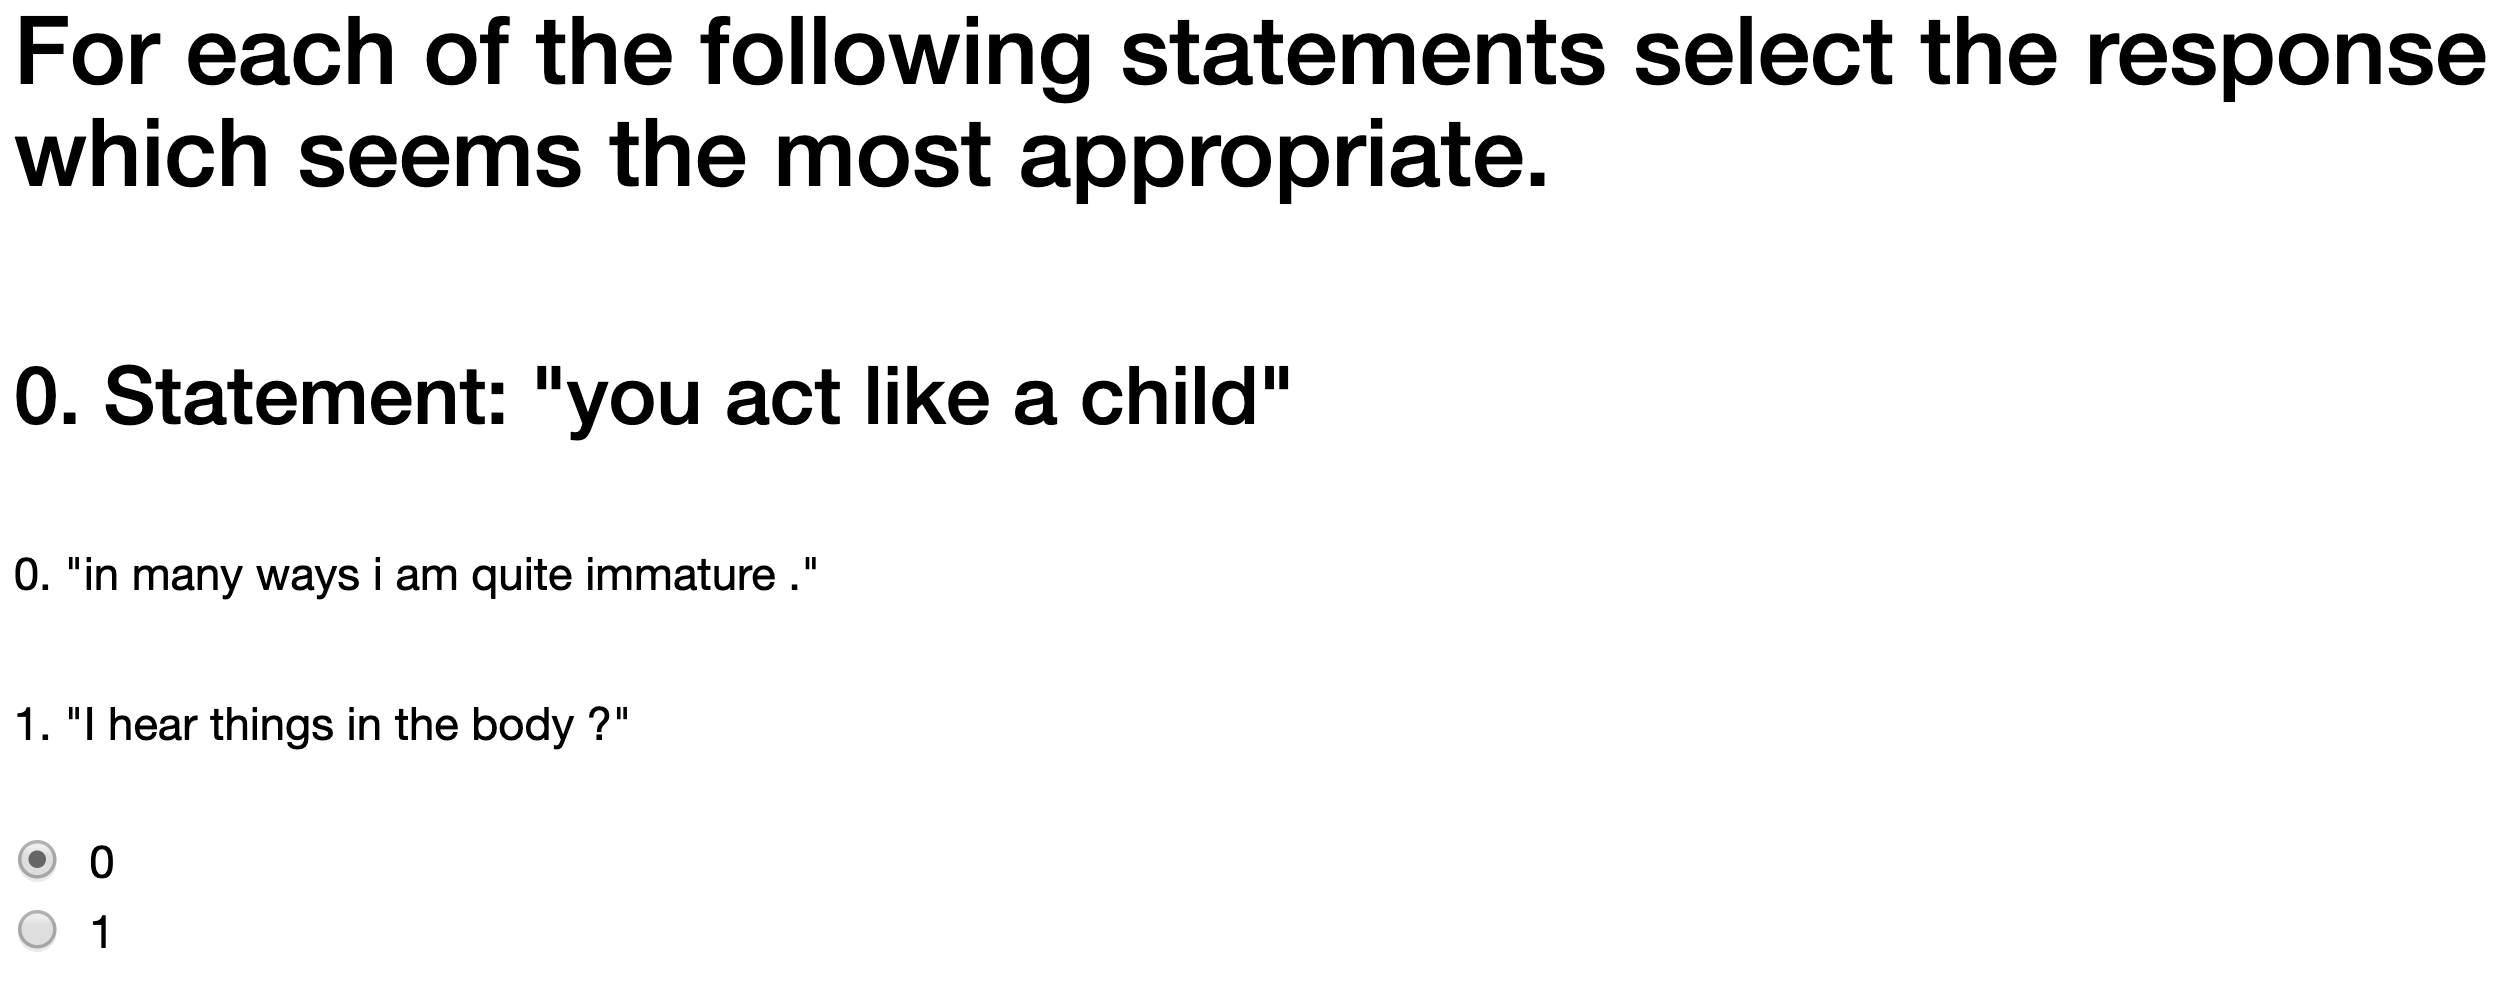
\includegraphics[width=\textwidth]{QuestionExample.PNG}}
	\end{center}
	\caption{Example of a question for the human evaluation metric.}
	\label{fig:human_eval_question}
\end{figure}
To evaluate the performance of our models we considered two types of metrics: a collection of automatic metrics and a human metric.
%For testing, we reserved $20\%$ of each datatset.
%These test sets were sampled at random from the raw dataset.
%As we will discuss later, we report both types of metric for each model and each test set independently.

The automatic metrics we considered were bilingual evaluation understudy (BLEU), recall-oriented understudy for gisting evaluation (ROUGE), metric for evaluation of translation with explicit ordering (METEOR) and word error rate (WER) \cite{Papineni:2002:BMA:1073083.1073135, lin-2004-rouge, denkowski:lavie:meteor-wmt:2014}.
These metrics are often used to evaluate the performance of translation bots and in some cases other chatbots.
However, despite a strong relationship between chatbots with personality and translation bots, these metrics are believed to be poor measures of performance for personality chatbots \cite{Radz2017, Xing2018, LiuLSNCP16, SerbanLCP15}.
Despite this, they are still often used to evaluate some aspects of a chatbot's performance.

The idea behind each of these metrics is to compared a response generated by one of our models against a saved test response.
The general idea behind BLEU, ROUGE and METEOR is to measure the overlap of words in the generated response and the test response.
The BLEU score is the normal BLEU score computed with weights $(.25,.25,.25,.25)$.
For ROUGE we report the  F1 score computed after calculating both the precision and recall.
We consider both ROUGE-1 and ROUGE-$\ell$.
We also collected additional ROUGE scores (e.g. ROUGE-$4$) but they were approximately $0$ for all of our experiments.
%A powerful tool for the METEOR metric is that it uses synonyms from a stored synonym library to extend this from exact word overlap to the overlap of closely related words.
We report the normal METEOR score.
All of these metrics output a score between $0$ and $1$ with $1$ being the best.
The WER metric computes the word edit distance between the generated response and the test response and outputs this divided by the length of the test response. 
For the WER score, a small number was best but the numbers could range to be arbitrarily large (if the generated response was very large compared to the test response).
We then average these scores over our entire dataset except for ROUGE which uses a corpus calculation.
We refer the reader to the appropriate references for a detailed explanation of these metrics.

For the human based evaluation we designed a jupyter notebook which randomly generated questions for each model from each dataset.
Each question had a test statement, test response and generated response.
The responses were placed in random order so that the tester would not know which was the generated response.
The tester was asked to select which response was most Joey like or appropriate for Joey to say given the response (See Figure \ref{fig:human_eval_question}).
We considered 4 testers familiar with Friends and the Joey character. 
Each tester answered at least 30 of these questions for each model and dataset combination.
For each tester and each combination, we calculated a final score by taking the total fraction of questions where the generated response was selected.
We then averaged them to get our final score for the combination.
Like the classic Turing test, an ideal outcome would be a score of $.50$.
That is, our model would create responses as Joey like as those from the actual show and the user would ultimately have to randomly pick between.



	
	\section{The Sequence-to-Sequence Model}
	%\section*{Why we tried this}
The first model we considered was a seq2seq (sequence-to-sequence) model.
It resembles the one mention in \cite{denkowski:lavie:meteor-wmt:2014}. 
While this architecture is usually used for language translation, it happens to also be widely used for chatbot creation. 
The success the seq2seq model has had in other chatbot implementations we researched, along with it's easy implementation in Keras is why this architecture was chosen.
In this section we discuss how we developed, trained and analyzed this model.

\subsection{Data Preparation}
%\begin{figure}
%\begin{python}
%	keepPunct = '[.,!?;]'
%	re.findall(r"[\w]+|"+keepPunct, 
%	'This is a test. Is this test 2?')
%	>>['This','is','a','test','.','Is','this','test','?']
%\end{python}
%\caption{Example of preprocessing statement for seq2seq model.}
%\label{fig:preprocess_s2s}
%\end{figure}
%\begin{python}
%	>>['<START> This is a test . Is this test ? <END>']
%\end{python}
Our first step was further reprocessing our datasets so that we could train on it.
We decided to do the following preprocessing steps:
%We break this process into the following steps:
We broke the dialogue into words  and punctuation mark. 
A word here does not have to reference and actual English word but a maximal sequence of characters excluding punctuation marks and white space. 
We decided that treating the punctuation marks as individual tokens would hopefully allow our model to better understand questions, statements and commands.
We also removed numerical data since smaller numbers were consistently represented by their word form and larger numbers seemed too rarely appear in the raw data.
This seemed like a easy way to reduce our vocabulary.
Finally we add a start and end tags to each statement.

To make the above data ingestible for the embedding layer of our model and easier to work with in general, every word, punctuation mark and tag was mapped to a numeric token. 
The \emph{tokenizer} consumes the entire corpus to create this mapping which is then applied to every statement and response in our dataset to create a collection of input and output sequence pairs.
The next was \emph{padding} the tokenized sequences with zeroes so they all have the same size.
%This was done by finding the longest sequence and padding all other sequences with zeros to have the same length as the longest sequence.
The input sequences were pre padded while the output was post padded.
%\begin{itemize}
%    \item When the sentence being processed is an output sentence a start and end token are added to the sentence.
%
%
%
%
%    
%\begin{python}
%    tokenizer = keras.preprocessing.text.Tokenizer(filters='\t\n',
%                                                   oov_token='<UNK>', 
%                                                   lower=False)
%    tokenizer.fit_on_texts(inputs + outputs)
%    tokenizer.texts_to_sequences(['This is a test input .',
%                        '<START> This is another test output . <END>'])
%    >>[[1,2,3,4,5,8],[10, 1, 2, 6, 4, 7, 8, 11]]
%\end{python}
%
%    \item 
%\end{itemize}
%\begin{python}
%    inputSequences = [[1,2,4,8],[2,4,3]]
%    ouputSequences = [[10, 1, 2, 6, 11], [10, 1, 2, 11]]
%    paddedInputs = preprocessing.sequence.pad_sequences(inputSequences,
%                                                     maxlen=maxInputLen,
%                                                     padding='pre' )
%    paddedOutputs = preprocessing.sequence.pad_sequences(ouputSequences,
%                                                     maxlen=maxOutputLen,
%                                                     padding='post' )
%    paddedInputs
%    >>[[1,2,4,8],[0,2,4,3]]
%    paddedOutputs
%    >>[[10, 1, 2, 6, 11], [10, 1, 2, 11,0]]
%\end{python}

Next, every token in the sequence had to be given a unique vector representation \cite{DBLP:journals/corr/MikolovSCCD13}. 
This was handle by a \textbf{keras.layers.Embedding} layer. 
To provide contextual representations of tokens (words, punctuation marks and tags), \textbf{GloVe 300-dimensional word embeddings} were used to initialized the embedding layer weights. 
Since the model outputs a \emph{softmaxed} prediction on each token, the next step involved converting output tokens to \emph{one-hot vectors}. 
Since the goal of the decoder was to predict the next token given the current token, the tokenized output sequence was shifted to the left by one step before being converted to one-hot vectors.  
%
%\begin{python}
%    #If the vocabulary was of size 3
%    paddedOutputs = [1,2,3,0]
%    paddedOutputs = paddedOutputs[1:] #left shift step
%    onehotOutput = keras.utils.to_categorical( paddedOutputs , 3+1)
%    onehotOutput
%    >>[[0,1,0,0],[0,0,1,0],[0,0,0,1],[1,0,0,0]]
%\end{python}

\subsection{The Model}
\begin{figure}
	\begin{center}
		\fbox{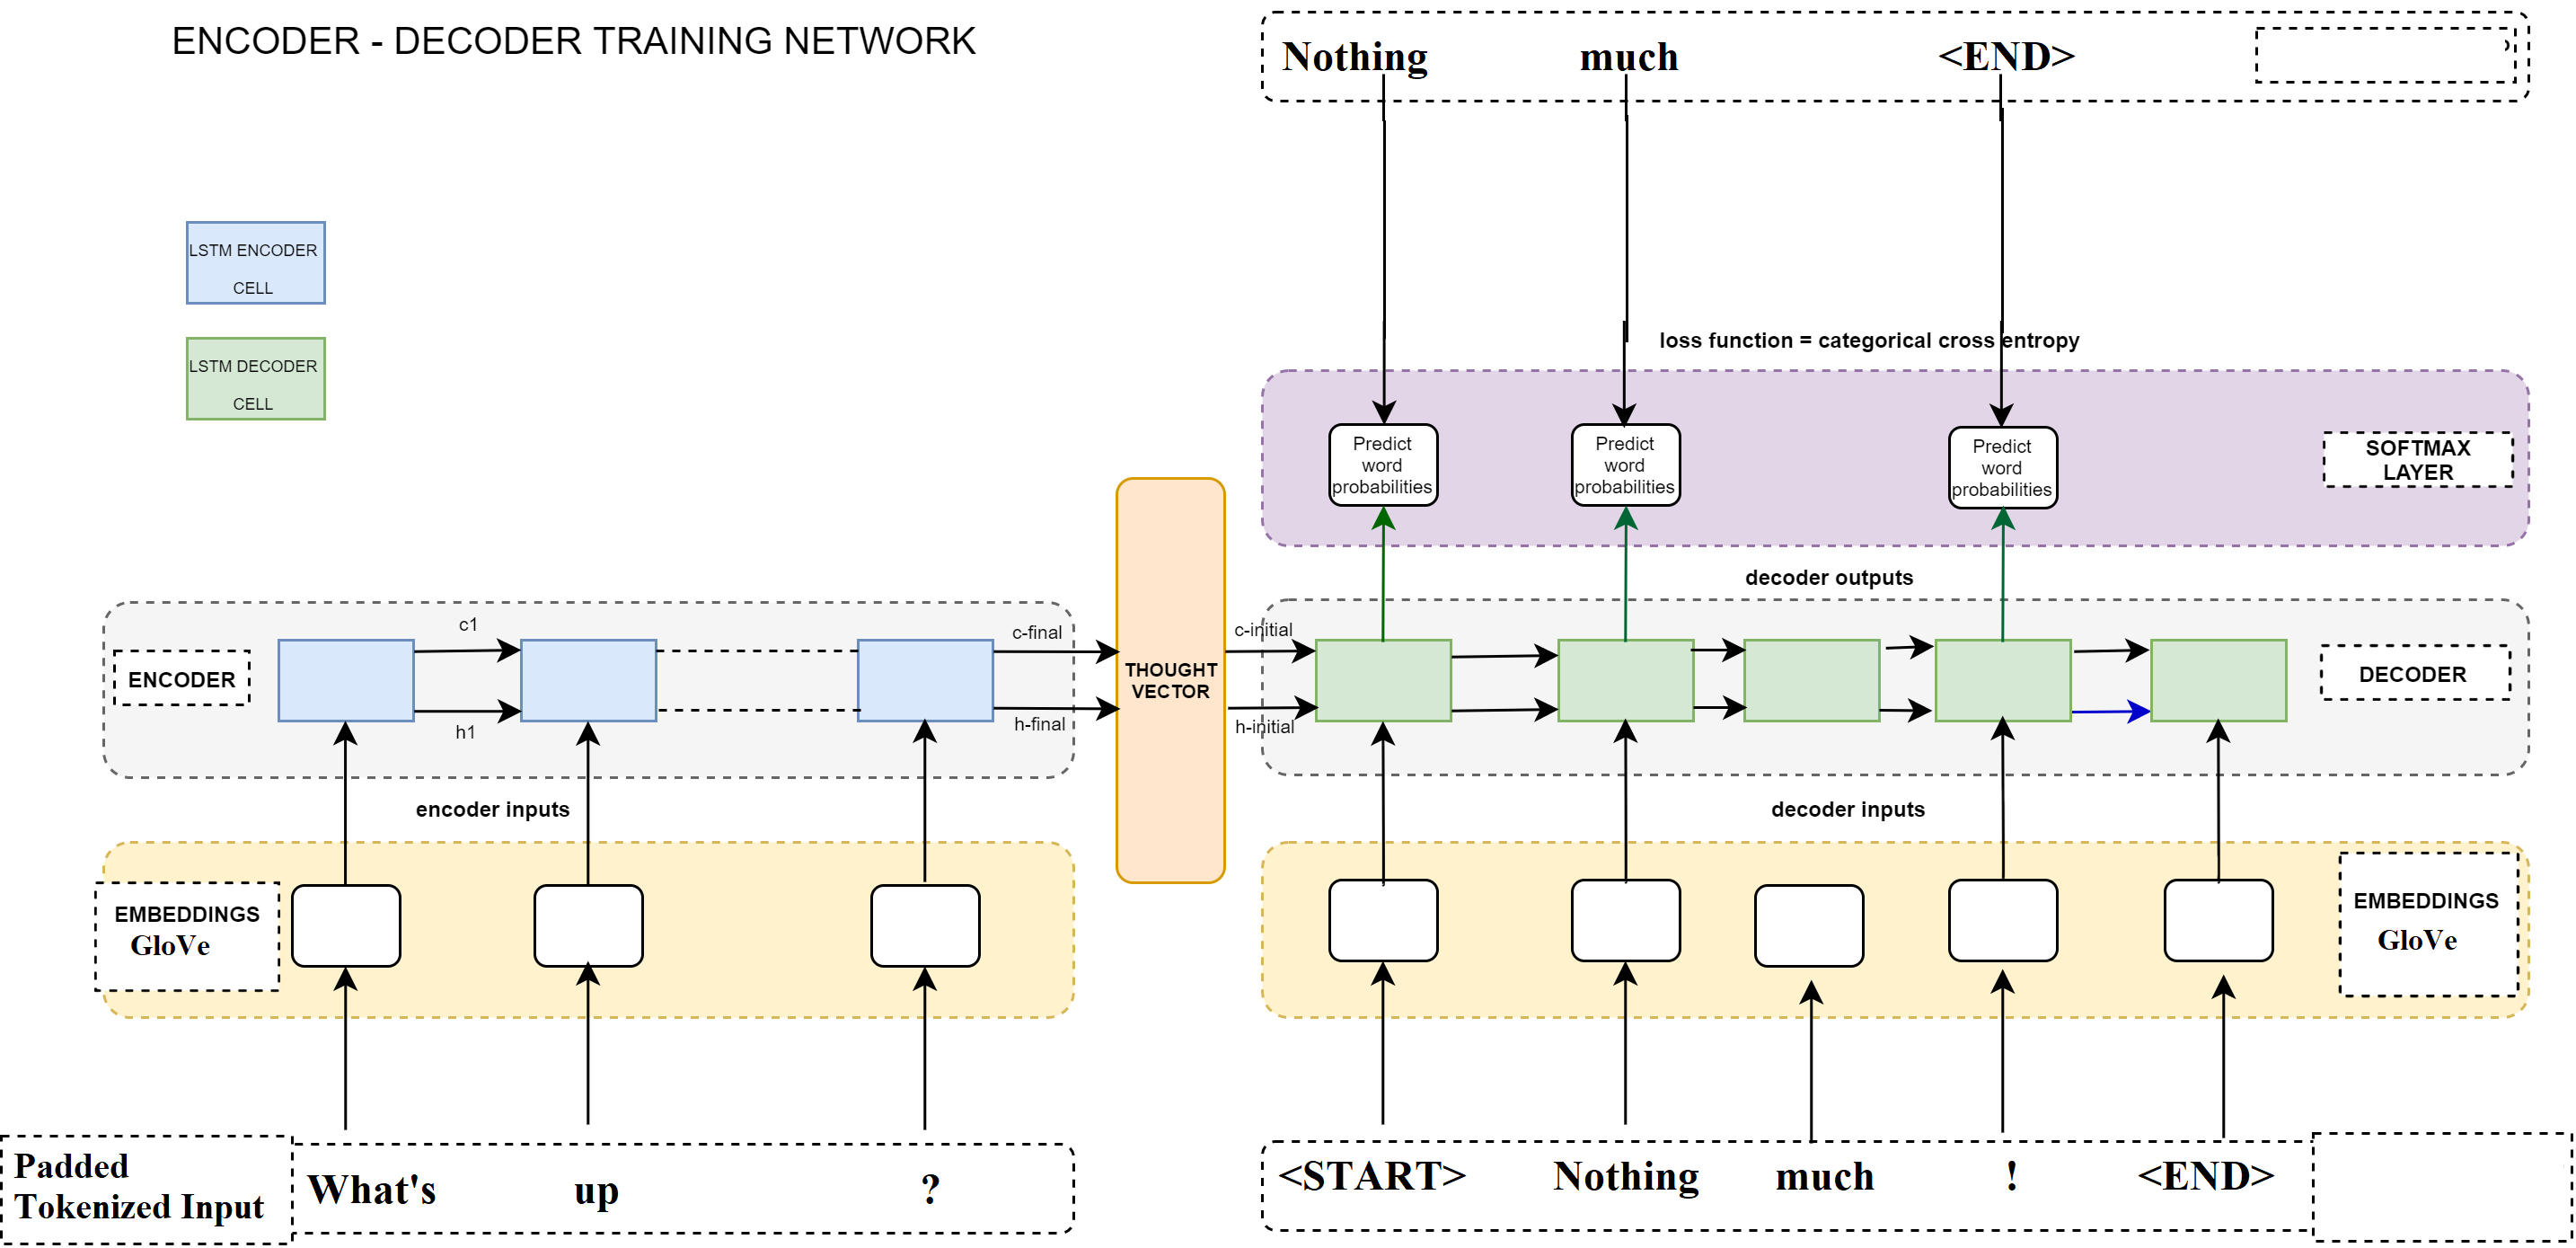
\includegraphics[width=\textwidth]{seq2seqModel.png}}
	\end{center}
	\caption{A diagram of our seq2seq model. Image edit from original image found \url{https://github.com/samurainote/Automatic-Encoder-Decoder_Seq2Seq_Chatbot.}}
	\label{fig:s2s_model}
\end{figure}
The model consists of an Encoder and a Decoder.
Padded input token sequences are converted to a sequence of word embeddings using a \textbf{Keras.embedding.layer} as described above.
Each of these word vectors are fed to the \textbf{keras.layers.LSTM} \emph{encoder long short-term memory} (LSTM) one at a time. 
The encoder LSTM tries to capture the essence of the encoded input sequence in two \emph{thought vectors}, the \emph{output context vector} and the \emph{hidden state vector}.
Both thought vectors are then passed to the decoder (See Figure \ref{fig:s2s_model}).

The \emph{decoder LSTM} is fed a padded sequence of output word embeddings along with the two thought vectors.
The decoder model is trained to use a \emph{dense SoftMax} output layer \textbf{keras.layers.Dense} with activation \textbf{keras.activations.softmax} to predict the most likely output word among all words in the vocabulary.
Once the model is trained, an \emph{inference encoder and decoder model} is created using the trained model weights. 
The inference encoder model takes in statement and two generated state vectors. 
The input state vectors are fed into the inference decoder model along with a sentence start tag. 
All words predicted by the SoftMax layer are captured until an end tag is generated (See Figure \ref{fig:s2s_model_decoder}).

\begin{figure}
	\begin{center}
		\fbox{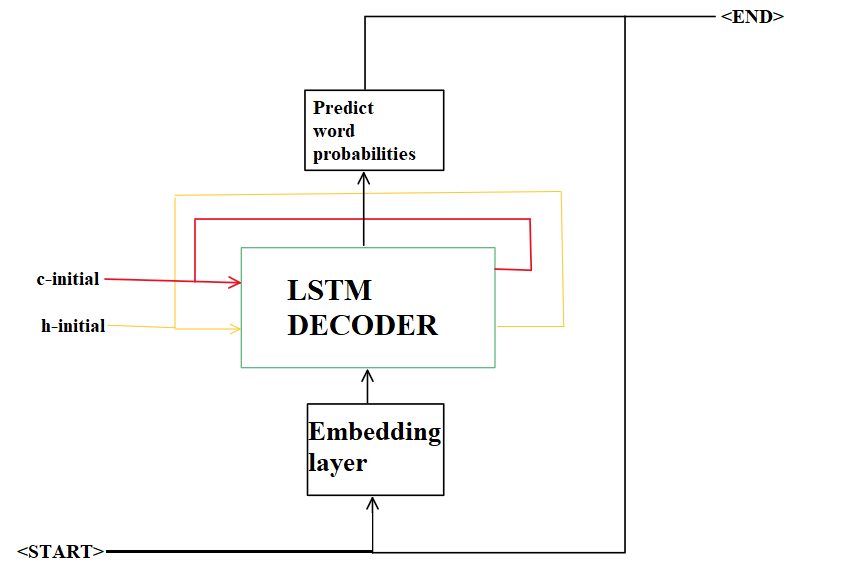
\includegraphics[width=.9\textwidth]{inference.png}}
	\end{center}
	\caption{A diagram of our seq2seq model's decoder.}
	\label{fig:s2s_model_decoder}
\end{figure} 

\subsection{Performance and Error Analysis}

\begin{figure}
\begin{center}
	\scalebox{.8}
	{
	\begin{tabular}{ |l|c|c|c|c|c|c|c| } 
		\hline
		\textbf{Dataset} & \textbf{BLEU Avg. Score} & \textbf{ROUGE-1 Score} & \textbf{ROUGE-$\ell$} & \textbf{METEOR Score} & \textbf{WER Avg.} & \textbf{Human Eval.}\\
		\hline
		Q\&A & $0.0530$ & $0.213$ & $0.204$ & $0.092$ & $1.554$ & $0.413$\\
		\hline
		Joey & $0.015$ & $0.141$ & $0.131$ & $0.064$ & $1.922$ & $0.350$\\ 
		\hline
	\end{tabular}
	}
\end{center}
\label{fig:s2s_data}
\caption{Table showing various scores for this sequence-to-sequence model on the Joey and generic questions and answers dataset (Q\&A).}
\end{figure}

\begin{figure}
\begin{center}
	\scalebox{.8}
	{
	\begin{tabular}{ |L|L| } 
		\hline
		\textbf{Question} & \textbf{Answer} \\
		\hline
		 Do you like food ? & I'm a software , I am an actor . I am , I am what am what am ? ! I am die of error ? \\
		\hline
	\end{tabular}
	}
\end{center}
\label{fig:s2s_errors}
\caption{Failure in generating grammatically correct sentence}
\end{figure}

As seen in Figure \ref{fig:s2s_data} this model did not perform well with respect to most of the automatic metrics.
This is somewhat to be expected though given that these types of metrics are known to be flawed when evaluating our kind of task.
We will discuss this in greater detail in Section \ref{sec:conclusion}.
We also note some success in this model for the human evaluation.
Again, these numbers may be slightly higher than expected due to the lack of preprocessing of our original dataset.
That is, some of it may be based on the human tester randomly picking between two poor responses to a statement and not necessary two equally good responses. 
We will also review this in greater detail in Section \ref{sec:conclusion}.

Here will review a few particular cases where this model consistently failed to perform well on human metrics and follow with some ideas for future improvement.

From Figure \ref{fig:s2s_errors} it is seen how the model fails to generate grammatically correct sentences. This is because, while the model understands how to mimic Joey, it seems to fail at understanding English grammar. This can be fixed by adding a \emph{conditional random field (CRF)} layer that uses the Viterbi algorithm. More detail is given about this in the next section.


\subsection{Pitfalls and Improvements}
One major pitfall faced while developing the seq2seq model was during training of our model. 
Specifically we initially had trouble providing the model with one-hot output vectors. 
As discussed above, the model uses a output softmax layer to predict the best possible word output. 
This means the length of each training output vector equals the length of the vocabulary of the entire corpus. 
This is multiplies by the number of tokens (words, punctuation marks and tags) in the sequence and this is then further multiplied by the number of training data points. 
With a vocabulary size of $3000$, a sequence length of $100$ and training data size of $7000$, the size of the entire output training data become $3000*100*7000$. 
This is too large of a matrix to store in memory. 
This problem was fixed by training in batches.
This was implemented using the Keras $fit\_generator$ function along with our own custom data generation function. 

One way we were able to imporove our model's performance was to change how we do our token embedding.
The initial model randomly generated embedding vectors of tokens. 
This did give good results as the word embedding held no information regarding the tokens they represented. 
This problem was fixed using GloVe word embedding that contextually represented the words they were associated to.
 
% During development, while training on a large number of epochs, a single failure in training lead to the loss of all training progress as the model was saved only in the end of training. 
% This was fixed by creating a custom Keras callback to save the model every specified number of epochs.
%\end{itemize}
%\section*{Future improvements}
While the current model seems to learn Joey like responses to some extent, it fails to understand how English sentences are structured. 
This leads to a lot of generated responses failing tests as they are eliminated for not looking like English sentences. 
We believe this can be fixed by adding a \emph{conditional random field (CRF)} layer using the Viterbi algorithm.
Hopefully this would give the model a better sense of English sentence structure. 
%This way a model know that an adverb comes after a verb etc. thereby facilitating the generation of English like sentences.
   
Another issue we noticed was that this model currently takes an argmax of the output predictions to choose the most probable word. 
Using a \emph{beam search} across predictions instead of just an argmax could improve prediction results.
    
The current model used just two fixed length vectors to represent the entire input sequence. 
When input sequence are really long, two fixed length vectors may not be enough to capture its entire essence. 
Attention could help solve this issue. 
The technique was tried but could not be successfully implemented due to the time constraint. 
Adding attention to models like this one has been show to drastically improve performance of the model when the input sentences are long.
	\section{Transformer Model}
	
	\begin{figure}[p]
	\begin{center}
		\fbox{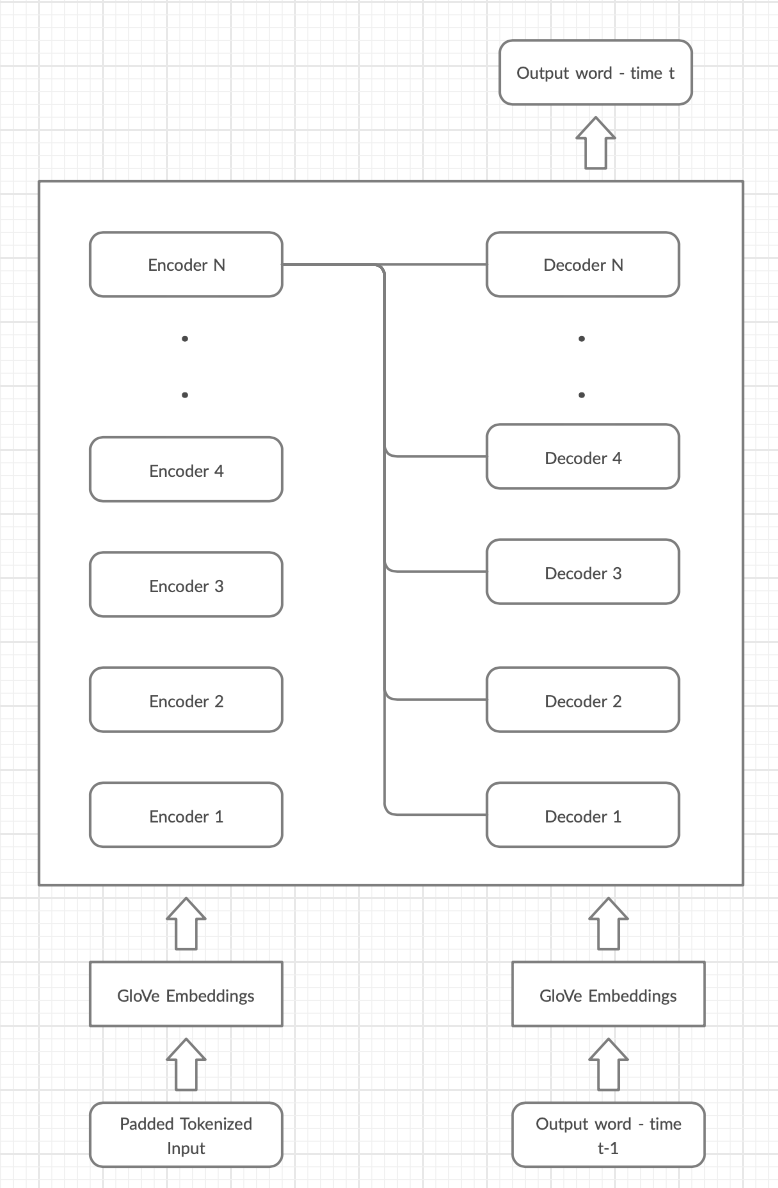
\includegraphics[width=1\textwidth]{TransformerImage.png}}
	\end{center}
	\caption{Transformer based Seq2Seq model.}
	\label{fig:trans_model_image}
\end{figure}

The second model we considered was another sequence-to-sequence model that used \emph{transformers} (See Figure \ref{fig:trans_model_image}).
The introduction of {transformers} in 2017 and it's success in \emph{natural language processing} tasks have caused it to replace LSTM \cite{DBLP:journals/corr/VaswaniSPUJGKP17}. 
The transformer performs better in retaining long-range context dependencies. 
It works on the self-attention mechanism. 
The recent performances of Google BERT (trained using transformers) and transformers in general motivated us to try it in our task.
In this section we discuss how we developed, trained and analyses this model.

\subsection{Model Architecture}

The Embedding layer uses the \emph{subword text encoder} from the Tensorflow datasets library. 
The architecture as shown in Figure \ref{fig:trans_model}, shows the structure of a single encoder-decoder unit. 
The units are designed such that the outputs of each encoder is connected to every decoder. 
The number of such units is a hyper-parameter.

The internal structure of the encoder contains a multi-head attention mechanism and a feed-forward network (See Figure \ref{fig:attention}). 
The multi-head attention network computes a series of scalar dot product attentions in parallel. 
This produces a base for enabling self-attention and sort of acts like an ensemble technique. 
The self-attention is computed using three vectors - \emph{query}, \emph{key} and \emph{value}. 
The weights for these vectors are learned during training. 
The dot product between each word embedding vector and each of these keys are used to compute self-attention. 
This process is done in parallel, multiple times. 
These outputs are concatenated and sent to the feed-forward network. 
The above process allows to jointly attend to information from different sub-spaces of representation.

The internal structure of the decoder is similar to the sub components of the encoder. 
The difference is the addition of a masked multi-head encoder. 
It is similar to the multi-head attention with a masking layer. 
The query vector to a decoder comes from the previous decoder layer while the key and value vectors come from the encoder network layers. The query, key and value vectors for the encoder units come from previous encoder layers. 
The decoder outputs from the feedfoward network is softmaxed over the vocabulary to produce the next probable word.

\begin{figure}[ht]
  \centering
  \begin{minipage}[b]{0.40\textwidth}
    \begin{center}
		\fbox{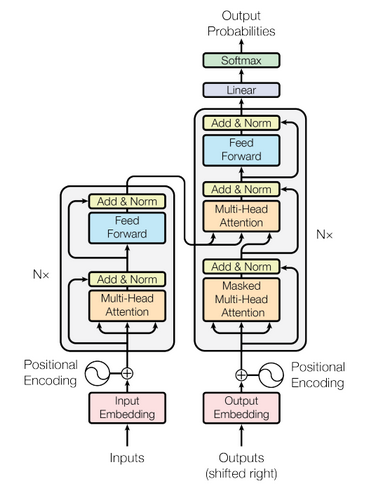
\includegraphics[width=\textwidth]{transformer.png}}
	\end{center}
    \caption{Encoder Decoder Unit. Image taken from \cite{DBLP:journals/corr/VaswaniSPUJGKP17}}.
    \label{fig:trans_model}
  \end{minipage}
  \hfill
  \begin{minipage}[b]{0.40\textwidth}
    \begin{center}
		\fbox{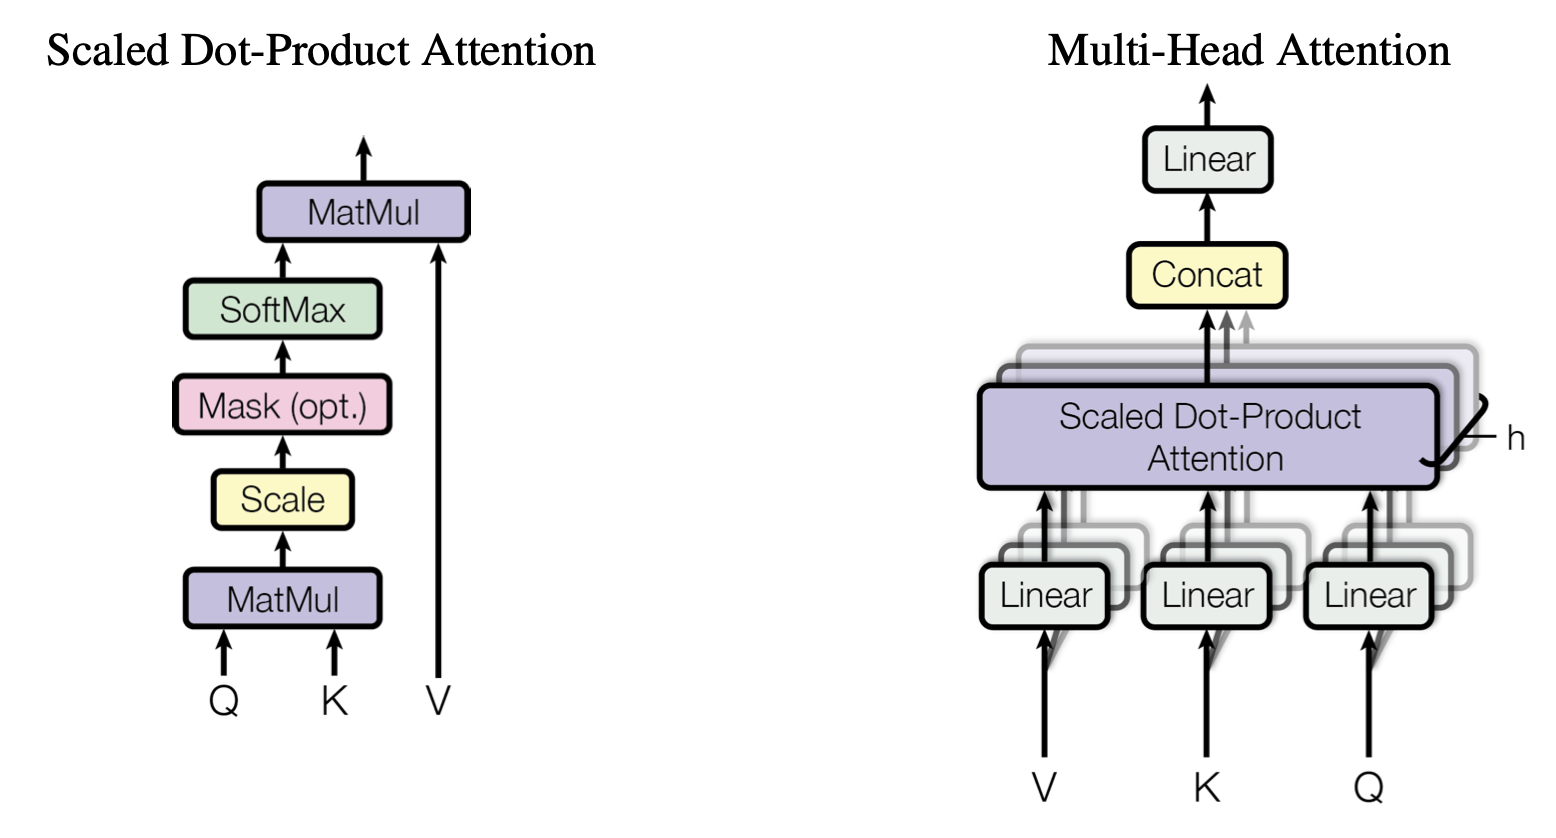
\includegraphics[width=\textwidth]{attention.png}}
	\end{center}
    \caption{Attention mechanism. Image taken from \cite{DBLP:journals/corr/VaswaniSPUJGKP17}}
    \label{fig:attention}
  \end{minipage}
\end{figure}

\subsection{Performance and Error Analysis}
\label{subsec:trans_s2s}
\begin{figure}[ht]
	\begin{center}
		\scalebox{.8}
		{
			\begin{tabular}{ |l|c|c|c|c|c|c|c| } 
				\hline
				\textbf{Dataset} & \textbf{BLEU Avg. Score} & \textbf{ROUGE-1 Score} & \textbf{ROUGE-$\ell$} & \textbf{METEOR Score} & \textbf{WER Avg.} & \textbf{Human Eval.}\\
				\hline
				Q\&A & $0$ & $0.102$ & $0.094$ & $0,035$ & $2.412$ & $0.263$\\
				\hline
				Joey & $0.110$ & $0.270$ & $0.0.261$ & $0.137$ & $1.218$ & $0.325$\\ 
				\hline
			\end{tabular}
		}
	\end{center}
	\caption{Table showing various scores for this sequence-to-sequence model with transformers on the Joey and generic questions and answers dataset (Q\&A).}
	\label{fig:trans_res}
\end{figure}
We note that the automatic metrics were run using our final trained models.
That is, we ran all the experiments  with a model trained first on the generic dataset and then the Joey dataset.
Based on the test results, both human and automatic metrics, the transformer model works better on the Joey dataset compared to the generic dataset.
One theory as to why this happened is that the transformer model performs better on datasets with large vocabulary and the generic questions and answer dataset has a very small vocabulary.
Moreover, we suspect that small size of the generic dataset compared to the Joey dataset may have been a big factor as well.

As we discussed in the previous section, considering a larger generic dataset may produce more promising results in final performance.
Just like the first sequence-to-sequence model, this model consistently generated response that did not parse as proper English sentences. 
%A review of the outputs produced on the generic test set will show that while responses are very different from the test response, they are still close just as close to English sentences (if not closer) compared to the original sequence-to-sequence model.
Future work could include trying to work on mapping how the model constructs a generic response and then tries to add 'Joey' characteristics to it. 
%Training the model on multiple datasets did not seem to solve this problem. 
We would suggest trying to add an additional learned component that tries to implement the idea of adding characteristics.
%Based on our initial test trials, we realized that the model is learning to respond based on a corpus entirely composed of the character's responses and has limited understanding of sentence formation. 
%Training the model on a general question answering corpus did not significantly increase the quality of sentences.
Therefore, a possible improvement to our model would be to train the model on a \emph{part of sentence task}. 
This might enable the model to learn sentence formulation mappings and could structure the sentences better.
%
%The Transformer model performs significantly better when the questions overlap contexts present in the television show. 
%The model generates responses that has fewer 'Joey' characteristics when asked generic questions than when asked questions with overlapping TV show context. 
%Overcoming this could be possible with the Part of Sentence training.

\subsection{Pitfalls and Improvements}
Some of the major roadblocks we faced during our implementation of this model included the construction of the transformer. 
There were no Keras or Tensorflow/PyTorch implementation of a basic transformer. 
Therefore, we had to refer to other sources to provide us with an implementations of the multi-head attention and positional encoding \cite{transmedium}. 

Another issue we faced was the inclusion/construction of context.
We tried to include the entire chat history (sequence of sentences processed previously) as a context vector to each computation. 
However, this idea did not increase the quality of results in \cite{DBLP:journals/corr/VaswaniSPUJGKP17} because the compilation of the entire history/context into a single vector doesn't seem to be effective. 
Therefore, we worked on producing output responses independent of previous context. 
Other sources (\cite{learndesmedium} and \cite{chatbotmedium}) indicate using the concept of goals/entities where the chatbot would recognize certain parts of the conversation as required entities (stored as context) and would work towards reaching a goal. 
This approach is quite specific and does not apply to general chatbots. 
We recognize this task as a possible area for future improvement.

	
	\section{Conclusion}
	\label{sec:conclusion}
	\subsubsection*{Acknowledgments}
	
	We would like to thank Chenhao Tan, Brian Groenke, Aakarsh Fadnis, and Madhusudhan Aithai Mahabhaleswhwara for their feedback on this project.
	
	\bibliography{references}
	\bibliographystyle{unsrt}
	
\end{document}